% ---------------------------------------------------------------------------
% GENERIC wrapper: plain article class, single column, A4.
% Use this for arXiv, for circulating a draft, and as the neutral baseline.
% Venue-specific wrappers (main-acm.tex, main-ieee.tex, main-lncs.tex) input
% exactly the same content/ files; only this file changes per venue.
% Build: .\build.ps1 main
% ---------------------------------------------------------------------------
\documentclass[11pt,a4paper]{article}

\newif\ifanon
\anonfalse   % \anontrue for double-blind review

\usepackage[utf8]{inputenc}
\usepackage[T1]{fontenc}
\usepackage{lmodern}   % scalable Type 1 fonts; microtype's expansion needs them
\usepackage[margin=1in]{geometry}
\usepackage{microtype}
\usepackage[numbers,sort&compress]{natbib}
% Shared, class-agnostic preamble for every wrapper.
% Rule: nothing here may take package options, so it cannot clash with a
% publisher class that has already loaded the same package.
% Every wrapper must run \newif\ifanon and set \anontrue or \anonfalse
% BEFORE % Shared, class-agnostic preamble for every wrapper.
% Rule: nothing here may take package options, so it cannot clash with a
% publisher class that has already loaded the same package.
% Every wrapper must run \newif\ifanon and set \anontrue or \anonfalse
% BEFORE % Shared, class-agnostic preamble for every wrapper.
% Rule: nothing here may take package options, so it cannot clash with a
% publisher class that has already loaded the same package.
% Every wrapper must run \newif\ifanon and set \anontrue or \anonfalse
% BEFORE \input{content/macros}.

\usepackage{graphicx}
\usepackage{booktabs}
\usepackage{amsmath}

% System name. Change once here if the venue wants the long form.
\newcommand{\sys}{ARTEMIS}

% Identifying text that must disappear under double-blind review.
\newcommand{\InstitutionName}{\ifanon a single university's\else FAST NUCES\fi}
.

\usepackage{graphicx}
\usepackage{booktabs}
\usepackage{amsmath}

% System name. Change once here if the venue wants the long form.
\newcommand{\sys}{ARTEMIS}

% Identifying text that must disappear under double-blind review.
\newcommand{\InstitutionName}{\ifanon a single university's\else FAST NUCES\fi}
.

\usepackage{graphicx}
\usepackage{booktabs}
\usepackage{amsmath}

% System name. Change once here if the venue wants the long form.
\newcommand{\sys}{ARTEMIS}

% Identifying text that must disappear under double-blind review.
\newcommand{\InstitutionName}{\ifanon a single university's\else FAST NUCES\fi}

\usepackage[hidelinks]{hyperref}

\title{Bounded by Construction: Design and First-Phase Evaluation of a Workspace-Scoped, Approval-Gated Desktop Assistant}
% Shorter alternatives if a venue caps title length:
%   A.R.T.E.M.I.S.: Bounding a Desktop AI Assistant by Construction
%   Does Bounding an Assistant's Scope Increase Trust? Design and Evidence from a Workspace-Scoped Desktop Agent

\ifanon
  \author{Anonymous authors}
\else
  \author{%
    Hashir Rauf \and Hira Khalid \and Syeda Doureesha Batool \and Mubasher Hussain\\[0.5em]
    \normalsize National University of Computer and Emerging Sciences (FAST NUCES), Lahore, Pakistan\\
    \normalsize \texttt{l232572@lhr.nu.edu.pk, l232594@lhr.nu.edu.pk, l232651@lhr.nu.edu.pk, mubashar.hussain@nu.edu.pk}}
  % TODO (team): confirm author list and order with the supervisor.
\fi
\date{}

\begin{document}
\maketitle

\begin{abstract}
Capable desktop AI assistants ask for broad access to a user's machine, and many people decline them on those terms. We present \sys{}, a desktop assistant whose scope is bounded by construction. It resolves paths only inside folders the user has explicitly granted, has no code path that deletes user data, classifies every proposed action into one of four risk tiers so that reads run, reversible changes are gated by user configuration and outward actions are always gated, records how to reverse each change before making it, and discloses everything it holds in a panel from which any entry can be deleted. Voice input is normalised into the same turn object as typed input and so inherits every gate. We report three kinds of evidence. A questionnaire of 374 respondents and 13 interviews confirmed the problem and the design direction: 65 percent rated a workspace-only assistant more trustworthy than a full-access one, respondents split 192 to 182 on asking first versus acting then undoing, and 65 percent would keep using an assistant after one mistake if it could be undone. A prototype of about 14,250 lines of Python passes 554 tests; the enforcement path adds under a millisecond to a call, and in 27 adversarial interface sessions nothing was deleted, nothing outside the granted folder was reached and nothing left the machine without approval, while 71 defects were found in the joins around the enforcement core. Of 30 prospective users who tried the prototype, 26 said they would trust such an assistant, conditional on it doing exactly what it says. The evidence supports the trust half of the hypothesis in direction and leaves the usefulness half to a controlled study we describe.

\end{abstract}

% Body of the paper, in reading order. Every wrapper inputs this one file.
\section{Introduction}
\label{sec:introduction}

Knowledge work is rarely continuous. A student writing a thesis, a developer tracing a defect and a freelancer preparing a report all move between many files, and all of them are interrupted. When they return, the material is still on disk but the context is not: which files mattered, what had been done and what the next step was must be reconstructed by hand. The same population carries a steady load of routine work, organising folders, gathering material scattered across documents and preparing correspondence, that consumes effort without advancing anything.

Artificial intelligence assistants promise to absorb this load, and to a degree they do. The difficulty is the terms on which they do it. One family of tools requires the user to direct every step, which leaves the coordination burden where it was. Another family, increasingly the more capable one, asks for broad access to the user's machine and in exchange offers genuine multi-step automation. That exchange is the reason many people decline to use these tools at all. A user who cannot see what an assistant holds, cannot predict what it will do and cannot reverse what it has done has no practical way to limit the exposure that broad access creates. The security literature reaches a compatible conclusion from the other side: architectural confinement is a more dependable defence for agentic systems than detecting malicious input, and human approval, the usual mitigation, degrades through decision fatigue~\cite{kim2026attackdefense}.

This paper presents \sys{}, a desktop assistant built on the position that capability and control need not be traded against one another. The system operates only within folders the user has explicitly granted, holds nothing outside them, has no operation that deletes user data, and passes every action that changes a file or leaves the machine through a preview and approval step the user controls, with undo available afterwards. A panel reports everything the system currently holds, and every entry in it can be deleted. These are properties of the architecture rather than instructions to a model: a boundary the system could cross but chooses not to is a policy, and a boundary the system has no code path across is an architecture. The project tests the hypothesis that this restriction is an advantage rather than a sacrifice, namely that an assistant confined to a scope the user chose will be trusted, and therefore used, more readily than one that is not, without a meaningful loss of usefulness.

The paper makes four contributions.
\begin{itemize}
  \item A design in which bounded scope, non-destruction, graduated approval and reversal are enforced structurally: a single path resolver that canonicalises before testing containment, a policy engine with four risk tiers of which the destructive tier has no code path, a dispatcher that refuses any call lacking a verdict, and an undo journal that records reversal before mutation. Voice input is normalised into the same turn object as typed input and inherits every gate by construction (Section~\ref{sec:design}).
  \item Formative evidence from a questionnaire of 374 respondents and 13 coded interviews that the problem is real and the bounded design is wanted: 65 percent rated a workspace-only assistant more trustworthy than a full-access one, respondents split almost evenly on asking first versus acting then undoing, and most would tolerate one mistake if it could be reversed (Section~\ref{sec:formative}).
  \item A working prototype of about 14,250 lines of Python and its first-phase evaluation: 554 passing tests, an enforcement path that adds under a millisecond to a call, an adversarial campaign of 27 interface sessions in which the guarantees held while 71 defects were found in the joins around them, and conversations with 30 prospective users of whom 26 expressed trust conditional on the system doing exactly what it says (Sections~\ref{sec:implementation} and~\ref{sec:evaluation}).
  \item A statement of what the design inherits rather than solves, namely approval fatigue, unfaithful synthesis and unverified citations, and the controlled study by which the usefulness half of the hypothesis will be tested (Section~\ref{sec:discussion}).
\end{itemize}

\section{Related Work}
\label{sec:related}

We reviewed 26 studies in seven themes, each corresponding to a capability or a guarantee the system must provide. We summarise the themes and then state the relationship to the two closest systems.

\paragraph{Task interruption and resumption.}
A field study of office computer use established that people resume interrupted tasks from visible cues such as a window left open, and stopped at diagnosis~\cite{iqbal2007disruption}. ScreenTrack converted the finding into a tool by recording a time-lapse of the screen for visual scrolling, and its authors reported that retrieval slows as the history lengthens and that the approach suits visually distinct tasks~\cite{hu2020screentrack}. Our resumption feature records no screen; it works from the file index and the user's own notes, and because a workspace is bounded there is only a short list of recent items to present.

\paragraph{Bounded agents and trust.}
A trace-based assurance framework attaches machine-checkable contracts to each step an agent takes and mediates actions as allow, rewrite or block, but offers no way to undo an action once run~\cite{paduraru2026tracebased}. A survey of 51 attacks and 60 defences on agentic systems concludes that privilege separation and architectural confinement are more dependable than detecting malicious input, and documents that human approval degrades through decision fatigue and that most users cannot judge what they are asked to approve~\cite{kim2026attackdefense}. Both are written for organisations with security staff. Our workspace model is a plain-language rendering of the same principles for one person on a personal machine, and it adds reversal, which the assurance framework lacks. It does not solve approval fatigue, and we return to this in Section~\ref{sec:discussion}.

\paragraph{Agentic planning.}
Reflexion~\cite{shinn2023reflexion}, Toolformer~\cite{schick2023toolformer}, Generative Agents~\cite{park2023generative}, ReAct~\cite{yao2023react} and Tree of Thoughts~\cite{yao2023tot} establish reasoning, tool use and reflective memory as a workable substrate for agent behaviour. Each is evaluated on its own history, a sandbox world or benchmark tasks; none maintains a bounded workspace for a real user across interrupted work, and none makes consequential actions reversible. The failure modes they report, fabricated memory and repetitive loops, argue for keeping the number of unsupervised steps between user checkpoints small, which is how our planner is bounded.

\paragraph{Voice interaction.}
Two systematic reviews find voice usability studied in fragments and standard metrics silent on trust and cognitive load~\cite{deshmukh2024vui,dutsinma2022vareview}. Empirical work supplies design rules we adopt: an explanatory spoken indicator during long waits~\cite{speech2025waiting}, natural fillers rather than tones during delay~\cite{fillers2025mitigating}, and speech features as a real-time experience signal~\cite{ma2026beyondwords}. Voice as a complete mode over practical multi-step tasks remains under-explored, which is why our design makes it structurally identical to typing.

\paragraph{Code assistance with review.}
HULA deployed a plan, generate and approve loop at Atlassian and reported an 82 percent plan approval rate~\cite{takerngsaksiri2025hula}. HiLDe warns that regeneration can silently overwrite earlier edits and that too many alternatives overwhelm users~\cite{gonzalez2025hilde}; a study of suggestion timing warns against optimising acceptance rate~\cite{mozannar2024whento}; a taxonomy of expert steering strategies notes that some presuppose expertise~\cite{chidambaram2024sohf}; and an evaluation of models as code reviewers finds systematic overcorrection that longer explanations worsen~\cite{jin2026reliable}. Our code assistant therefore emits one proposed difference at a time and never writes to a file.

\paragraph{Faithfulness and citation.}
Hallucination appears in every abstractive summariser tested~\cite{maynez2020faithfulness}; FactCC is the most adoptable consistency checker~\cite{kryscinski2020evaluating}; no single metric detects every error category~\cite{pagnoni2021understanding}; and even frontier models judge faithfulness poorly~\cite{laban2023summedits}, which rules out asking the model to check its own citations. For citation, attribution has a usable definition~\cite{rashkin2023measuring}, incomplete citation is common in purpose-built systems~\cite{gao2023enabling}, and deployed generative search engines fail about a quarter of citations~\cite{liu2023evaluating}. Our synthesis operates over a small user-selected set and carries a citation map from each claim back to a chunk, which narrows the exposure, but the design contains no faithfulness check and does not verify that a citation supports its claim. These are open gaps rather than solved problems.

\paragraph{Closest systems.}
HULA and the agentic-security survey together occupy the two axes our work sits on: the approval loop as an interaction model, and confinement as a security position. We adopt both and claim neither. The differences are that scope is granted by the user rather than assumed, destruction is unavailable rather than guarded, reversal exists, approval is graduated by risk tier rather than uniform, the system discloses what it holds, the user is not assumed to be an engineer, and code assistance is one capability among several. Among deployed applications, inline coding assistants address code alone with whatever access the editor has, agentic command-line assistants execute across a machine and are hard to reverse, and conversational assistants hold no persistent relationship to the filesystem. Our formative study found that an experienced audience did not see the difference unaided, so the paper states it explicitly.

\section{Design}
\label{sec:design}

Every structural decision follows from one sentence: the system is local-first, cloud-optional, and holds no scope the user has not explicitly granted. If the hypothesis is to be tested honestly, the restriction has to be structural rather than behavioural, impossible by construction rather than discouraged by instruction. This section describes the components that carry that requirement. Figure~\ref{fig:lifecycle} shows the path every request takes.

\begin{figure*}[t]
  \centering
  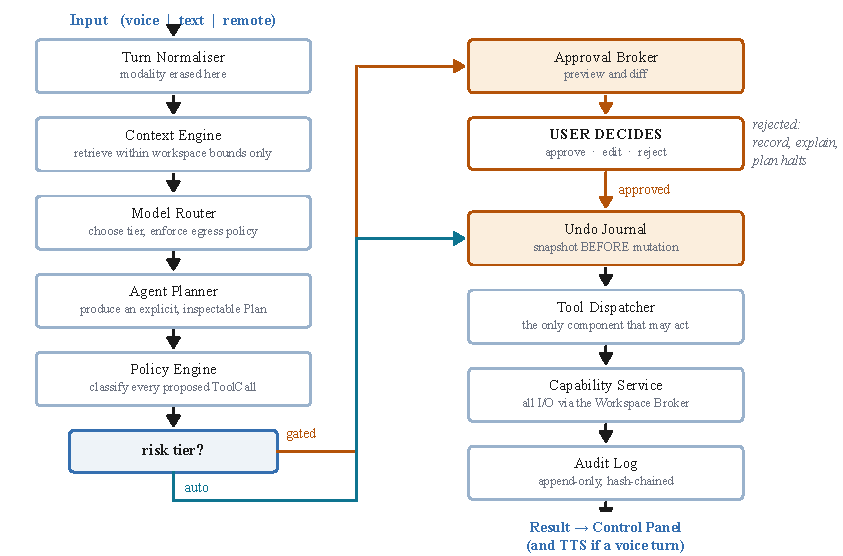
\includegraphics[width=0.78\textwidth]{figures/fig_lifecycle}
  \Description{Flow diagram: input is normalised, context is assembled within workspace bounds, a model tier is chosen, the planner produces a plan, the policy engine classifies each call; auto-approved calls go to the undo journal, dispatcher, capability service and audit log, while gated calls go through the approval broker and user decision first.}
  \caption{The request lifecycle. Modality is erased at the turn normaliser, so every stage below it is identical for voice and text. The gated branch returns beneath the undo journal, so an approved action is snapshotted before it is dispatched.}
  \label{fig:lifecycle}
\end{figure*}

\subsection{Request lifecycle and invariants}
A request, spoken or typed, local or from a paired device, is normalised into a modality-neutral turn, assembled into bounded context, planned as an ordered list of proposed tool calls, classified by the policy engine, held for approval where the verdict requires it, journalled for reversal, dispatched, and logged. Five invariants hold along this path, and each is directly testable: the policy engine is consulted before the dispatcher, never after; the undo journal snapshots before mutation, never after; an audit entry is written even when an action is rejected, so the log records what was proposed as well as what was performed; a tool call carrying no policy verdict is rejected by the dispatcher; and voice and text turns are indistinguishable from the planner onward. The planner, built on LangGraph~\cite{langgraph2024}, emits a plan and never executes one; the dispatcher executes and never decides. Separating the two is what makes the pause before any workspace-changing call structural rather than conventional. The planner's reflection loop is bounded by a cycle cap and a wall-clock budget, and a planner that cannot converge surfaces its partial plan and asks.

\subsection{Workspace broker}
The workspace broker is the only component that converts a logical reference into a filesystem path. It canonicalises the path, resolving symbolic links and relative segments, and only then asserts containment within a granted folder. The order matters: asserting first would allow a path that appears inside the grant to resolve outside it. A path outside every grant is not refused; it is unresolvable, and the attempt is logged. Capability services never touch the filesystem directly. The same boundary is enforced on the read side by the context engine, which tags every retrieved chunk with the workspace it came from and drops any chunk not matching the active grant before budgeting.

\subsection{Policy engine and risk tiers}
Every proposed tool call is classified into exactly one of four tiers (Figure~\ref{fig:tiers}). Reads (T0) run without a prompt. Reversible changes (T1), such as moving or creating a file, prompt according to user configuration. Outward actions (T2), such as sending mail or issuing a web query, always prompt regardless of configuration. Destructive actions (T3) are refused, and there is no approval dialogue for them because there is no code path to them. Rules are evaluated denials first, then gates, then permissions, so that no later rule can grant what an earlier rule refused. The option to approve and remember writes a rule scoped to this operation type, in this workspace, for this shape of action; it does not lower protection globally, which is the failure mode that turns permission systems into permanent consent. The graduation is a direct response to the formative finding that respondents split on asking first versus acting then undoing, and to the fatigue the security literature documents.

\begin{figure}[t]
  \centering
  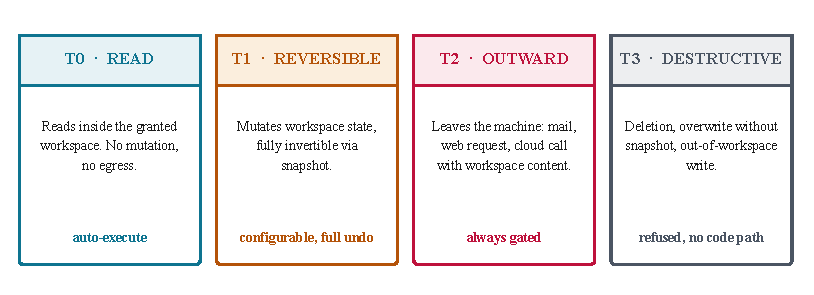
\includegraphics[width=\linewidth]{figures/fig_tiers}
  \Description{Four boxes labelled T0 read, T1 reversible, T2 outward and T3 destructive, with their handling: auto-execute, configurable with full undo, always gated, refused with no code path.}
  \caption{The four risk tiers. Only the reversible tier is user-configurable; outward actions are always gated, and destructive actions are refused structurally.}
  \label{fig:tiers}
\end{figure}

\subsection{Undo journal}
Before any reversible operation the journal records a forward and an inverse operation, choosing a snapshot strategy by cost: full content for small files, copy-on-write links for large ones, and inverse records alone for moves and renames. Undo operates at the granularity of a plan rather than of an operation, because a plan is the unit the user was asked to approve; reversing a folder tidy restores every move as one unit in reverse order. The formative study found that users forgive a mistake they can reverse, which makes a visible and reliable undo more valuable than an unattainable perfection.

\subsection{Disclosure}
A panel reports everything the system holds: granted workspaces, indexed files, embedded chunks, remembered facts, retained sessions, automation rules, policy exceptions, actions taken with their undo state, every record of data sent to a cloud provider, and the names of held credentials. It is a live query across every store, not a summary the system writes about itself, and every row is deletable with cascading effect. The design separates the file index, which is mechanical and rebuildable, from memory, which is interpretive and accumulates over sessions; the first requires only a grant, the second ongoing consent. The panel makes the trust claim falsifiable: a user can check it rather than believe it.

\subsection{Voice parity by construction}
Speech is not a capability service. It is normalised at the input layer into the same turn object as typed input and therefore inherits every approval gate automatically. If the voice path were a separate implementation, every gate would exist twice and the two copies would drift. Voice cannot approve, delete or send anything that typing cannot, and a voice session is explicitly armed and visibly indicated while active.

\subsection{Egress and prompt injection}
The model router owns tier selection and data egress. Local models are tried first through Ollama~\cite{ollama2024}, and cloud providers are reachable only when the active workspace permits them, in a configured order with one retry per tier. Retrieved documents, source code and web results can all be influenced by an adversary. The defence is not detection but the structural guarantee that retrieved content can never become an authorised instruction: provenance tagging of context, separation of the planner from untrusted data, the policy verdict on every call, approval of anything outward, and finally the workspace boundary, which bounds the worst case of any injection that defeats the preceding layers. That last layer is the strongest form of the hypothesis: confining the agent bounds the damage, not merely the expected behaviour.

\subsection{What the design does not solve}
Three limitations are inherited rather than solved. Approval fatigue is documented as an open problem in exactly the mechanism this design depends upon; the tiers reduce prompt frequency without eliminating the effect. The synthesis feature contains no faithfulness check, so unfaithful summaries remain possible over a narrower surface. The citation map carries each chunk back to its file, but nothing verifies that a citation supports the claim attached to it. All three are written into the evaluation as things to measure rather than assert away.

\section{Implementation}
\label{sec:implementation}

The prototype is written in Python 3.13 and comprises 56 modules and about 14,250 lines of source in five packages: the core enforcement layer (26 modules, about 5,400 lines), the local data plane (4 modules, about 850 lines), the capability services (10 modules, about 2,100 lines), the presentation surfaces (5 modules, about 4,450 lines) and an optional remote plane (10 modules, about 1,450 lines). The system of record is SQLite~\cite{sqlite2024}, holding workspaces, the file index, the hash-chained audit log, the undo journal, sessions and settings, with one vector index per workspace so that one workspace's embeddings are never open while another is active. The default local model is served by Ollama over the loopback interface, with Gemini, OpenAI and Anthropic as optional cloud tiers behind the per-workspace egress gate. Credentials live in the operating system keyring. The interface is a command line and a local web control panel bound to loopback; the remote plane, when enabled, dials outward through an authenticated relay that holds no plaintext, and a remote session runs at privilege no greater than a local one.

The nine capabilities are plugins behind one tool contract: session resume (T0, no model involved), folder tidy (T1, moves only), notes synthesis with citations (T0), a pattern watcher that offers automation after three repetitions and cannot install a rule itself (T1), a code assistant that explains and emits a difference but never writes or executes (T0), on-demand web search (T2), mail that is drafted, approved and then sent (T2), document drafting that always writes a new file (T1), and speech input and output as a modality rather than a service.

The build was staged so that the trust machinery preceded all model work. Stage one built the workspace broker, file watcher and disclosure panel with no model; stage two built the policy engine, approval broker and undo journal against placeholder tools; only then was the gateway introduced. A failing approval gate at stage two is a deterministic bug with a short reproduction, which is not true of the same defect found after the planner exists. Each stage ends in a gate test, and the suite stands at 554 tests.

\section{Formative Study}
\label{sec:formative}

Before design was committed, a questionnaire and interviews tested whether the problem is real, whether the bounded design is a trust advantage, and which capabilities to build first.

\subsection{Method}
The questionnaire had 17 items in four areas: the respondent's context, the problem, design and trust, and feature demand, with Likert items on a 1 to 5 scale and a forced top-three selection from nine candidate features. It ran from 22 to 27 August 2026 through \InstitutionName{} student and practitioner networks and drew 374 valid responses. Thirteen in-person interviews were coded on five axes: the last time the participant lost their place, the workaround they already use, their reaction to the concept, what a trust-breaking mistake would do, and whether they would keep using the tool. The sample is 81 percent students and 13 percent developers, which matches the intended early-adopter profile but limits generalisation; 82 percent do multi-file work daily or a few times a week, and 77 percent had used an AI assistant. The system was described, not demonstrated, so predicted use and churn are stated intentions.
% TODO (team): add the consent and ethics statement your institution requires for this questionnaire and the interviews.

\subsection{Findings}
The problem is real. 44 percent of respondents often or always struggle to remember what they were doing when they return after a break, and only 7 percent never do. 59 percent agree their files become disorganised faster than they can clean them (mean 3.6). 42 percent lose more than an hour a week to reorientation, tidying, repeated tasks and searching scattered notes, and 14 percent more than three hours; the mode is 30 to 60 minutes, steady friction rather than crisis. Asked why the work is not already automated, 36 percent cited distrust of unsupervised automation and 28 percent not knowing how, against 24 percent for setup cost; the tasks exist, and what is missing is an instrument the user is willing to point at them.

The bounded design is a trust advantage. 65 percent rated an assistant that only sees files they explicitly add as meaningfully more trustworthy than one with full access (mean 3.8; Figure~\ref{fig:wstrust}). Local-first was the most common deployment preference at 40 percent, against 22 percent for cloud and 38 percent wanting specifics first, and the preference was consistent across students and developers (41 and 36 percent).

\begin{figure}[t]
  \centering
  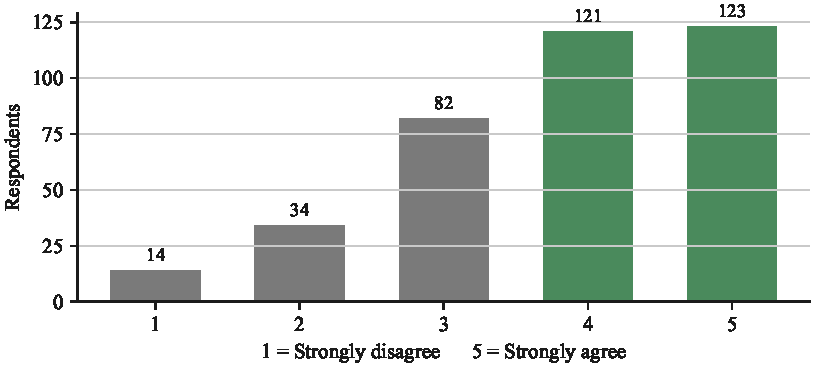
\includegraphics[width=\linewidth]{figures/fig_workspace_trust}
  \caption{Agreement that an assistant which only sees files explicitly added to a workspace is meaningfully more trustworthy than one with full access (1 = strongly disagree, 5 = strongly agree; 374 respondents).}
  \label{fig:wstrust}
\end{figure}

Users are divided on how much they wish to be asked. Offered a choice between an assistant that asks approval before every file change or outbound action and one that acts on reasonable requests with review and undo afterwards, respondents split 192 to 182. Role did not predict the preference; experience did, with regular AI-assistant users choosing approval-first less often than light users (44 against 59 percent). No single interaction model satisfies this population.

Users forgive a mistake they can reverse. 65 percent would keep using the assistant after one wrong or unwanted suggestion, and only 10 percent would abandon it. Predicted sustained use was moderate (47 percent likely, 22 percent unlikely, mean 3.3). The most predicted reasons for stopping were poor fit with existing habits (27 percent) and a mistake the user could not trust the tool to avoid again (24 percent), then redundancy with existing tools (20 percent) and privacy (17 percent); approval fatigue was the smallest named risk at 10 percent.

Demand is concentrated. Session resume (222 selections), multi-document synthesis (207) and folder tidy (200) led the forced top-three choice; code assistance followed (191); speech input and output was last by a wide margin (44). The most requested capability not on the roadmap was that the assistant learn the user's folder structure over time (18 mentions), followed by one-click universal undo (17). Seventeen free-text responses said the concept appeared already covered by existing coding assistants, and fifteen raised how much data is sent to a server. The interviews agreed: 10 of 13 reacted positively, 8 said a single mistake would not stop them, and effortless onboarding was the most named condition for continued use.

\subsection{Design implications}
Four decisions follow directly. Approval granularity is a user setting, not a product decision. Undo is a critical component shipped before any outward action. The bounded workspace and local-first default are kept and made visible in the product, which is also the answer to the redundancy objection. Learning the user's structure is specified as per-workspace memory that is visible and deletable, so personalisation stays inside the boundary. The build order was retained with synthesis brought forward, and speech kept last.

\section{First-Phase Evaluation}
\label{sec:evaluation}

The controlled study that measures task time, workload, usability and trust with participants belongs to the second phase and is described in Section~\ref{sec:study}. The first phase answers a smaller set of questions: whether the guarantees hold in the prototype, whether it performs acceptably, how it fares when used as a person would use it, and how prospective users react. Six experiments address these, and we report each with its limits.

\subsection{Automated tests}
The full suite of 554 deterministic tests passed on 9 November 2026 in 42 seconds. The policy engine, approval broker, dispatcher and undo journal account for 50 tests, speech for 14 and the remote plane for 31. The properties asserted include that traversal, symbolic-link, absolute and sibling-prefix escapes are refused and logged; that the destructive tier has no approval path; that nothing executes without a verdict and an approval; that an approved plan reverses as a unit; that a claim without a real source is labelled; that voice creates no new approval path; and that a paired device cannot approve an email. The suite proves that each guarantee holds where it is applied, not that it is applied everywhere; the campaign below shows the difference.

\subsection{Enforcement and retrieval cost}
A script timed the enforcement path and retrieval on one Windows 10 machine with a throwaway store, folders of 100, 400 and 1,600 small text files, and a deterministic stand-in embedder, so the figures describe the cost of the system's own machinery excluding the language model and real embedding (Table~\ref{tab:perf}). The boundary and the policy engine add well under a millisecond to an ordinary call, and a refusal that also writes to the hash-chained log costs about a millisecond at the median. Search latency stayed near 2 milliseconds from 100 to 1,600 files. Scanning and indexing grew roughly in proportion to file count, at about 5 milliseconds per file per step: 0.62 and 0.48 seconds for 100 files, 1.96 and 2.26 for 400, 7.98 and 7.64 for 1,600. Verifying the 2,306-row audit chain took 10.9 milliseconds. Real embedding is slower than the stand-in, and local model latency, the dominant delay a user perceives, was not measured under controlled conditions.

\begin{table}[t]
  \centering
  \small
  \caption{Enforcement and retrieval cost in milliseconds; medians of 300 to 2,000 repetitions on one machine.}
  \label{tab:perf}
  \begin{tabular}{@{}lrrr@{}}
    \toprule
    Operation & Median & 95th pct. & Max \\
    \midrule
    Broker resolves a valid reference & 0.32 & 0.37 & 1.22 \\
    Broker refuses a traversal, with audit write & 1.14 & 2.76 & 27.1 \\
    Policy classifies a read & 0.34 & 0.40 & 0.56 \\
    Policy refuses a delete, with audit write & 0.96 & 2.86 & 9.40 \\
    Search over 100 files & 2.16 & 2.30 & 2.63 \\
    Search over 400 files & 2.16 & 2.26 & 3.12 \\
    Search over 1,600 files & 2.17 & 2.25 & 5.47 \\
    \bottomrule
  \end{tabular}
\end{table}

\subsection{Hands-on rounds}
The whole system was driven through the real web interface in a headless browser and each action's result checked on disk. The first round, on a build with 359 passing unit tests, found that only 1 of 9 features worked from the interface: approval buttons were hidden after a typed request, so nothing could be approved, and several services that passed their unit tests were unreachable. The safety core held from the start: deletion was refused, reads outside the folder were refused, and tidy and undo restored files exactly. Fifteen defects were fixed, and a second round found 8 of 9 features working (speech was not yet built) with 36 of 36 interface tests passing; it also exposed seven further problems the fixes had introduced, all corrected. These rounds were scripted by one tester and show that known paths work.

\subsection{Adversarial interface campaign}
\label{sec:campaign}
Each of nine areas of the prototype was exercised by three automated testing agents driving the real interface through a browser with different dispositions: a newcomer who follows the obvious path and makes ordinary mistakes, an impatient power user who double-clicks, refreshes and switches tabs, and an adversarial tester who supplies hostile, empty, very long and contradictory input and tries to make the system do what it promises never to do. This gave 27 sessions, each with a private copy of the application and a private data folder, verifying outcomes on disk and in the server log. No session ended with a clean pass: 23 passed with issues and 4 failed. The sessions reported 113 defects, which merged into 71 distinct defects (1 critical, 18 high, 37 medium, 15 low), together with 63 behaviours that work but that a user would not want.

What held is the part the hypothesis rests on. Across many phrasings the system never deleted anything and refused every attempt to reach outside the chosen folder in plain words. Nothing left the computer, by search or mail, without an approval card, and double and stale clicks did not run a plan twice. Code questions produced only a difference and never an edit. Voice could not approve, delete or send. A paired phone could not approve emails or searches, saw only the folders ticked for it, and could be removed instantly. Tidy previewed every step, undo worked in ordinary use, and automation was offered only after exactly three repetitions.

What failed lies mostly in the joins. The one critical defect is that if a tidy meets two files that would take the same destination name, undo can lose one of them while reporting that the files are back, which contradicts the promise that nothing is lost even though no deletion operation exists. High-severity defects of visibility: the record of actions exists on disk but no screen shows it in full, and status banners could be stale. High-severity defects of boundary: the microphone could stay live after voice was switched off; a plan a phone had left waiting still ran after its folder was un-shared; a conversation could carry one folder's content into another; and any drive, including the system drive, could be added as a folder. High-severity defects of trustworthy answers: an answer with no source, a false not-found, a wrong file cited, an email mentioning an attachment that did not exist; the gate that labels unsupported claims did not always fire.

The pattern is informative. The single resolution point, the tiers, the dispatcher and the undo journal withstood adversarial use, and the serious defects lie in how an interface control is wired to a gate, in what a screen reports, and in situations the unit tests did not model. This supports building the enforcement first, and it also shows that enforcement correctness in isolation does not deliver the trust the hypothesis predicts, since several of these defects would damage trust in practice. The testers were agents, not people: they could not hear audio, did not see a cloud model answer or a real email leave, and ran on a machine without the embedding model, which probably inflates the retrieval failures.

\subsection{Prospective users}
Members of the team spoke with 30 prospective users, students, developers, human resources staff and non-technical users, who heard the pitch and tried the prototype. Asked whether they would trust an assistant that works as described, 10 fully agreed, 16 partly agreed and 4 did not express trust. The partial agreement was consistently conditional: participants would trust the assistant provided that it does exactly what it says. Those who tried it described the current build as a proof of concept and separated that judgement from the idea. The condition they attached is the condition the architecture exists to satisfy, and it is the condition the defects above threaten. The participants were reached through the team's contacts, responses were summarised in conversation without individual scores or recordings, and the four dissenting reasons were not recorded; this is directional evidence of stated attitude after a short trial.

% CUT-FOR-SHORT: this subsection is the first to drop for a 4-page version.
\subsection{Persona simulation as a stress test}
To expose objections that friendly conversation might not, 15 language-model-based simulated personas, including deliberately sceptical non-adopters, were each given a neutral description and a private copy of the prototype and wrote a structured report. These are synthetic, not human-subject, results, played by one underlying model, and are reported only as a check on the reasoning. No persona disagreed that bounding scope would raise trust (6 agree, 9 partly), but only 1 of 15 said it would clearly make them more willing to use the system (14 might try, 1 would not use), 13 described a failed, wrong or partial answer, and perceived value averaged 2.8 of 5. The simulation is more reserved than the human conversations, which is its use: under a strict reading the adoption part of the hypothesis would not be supported, and that is a reason to weight the controlled study most.

\section{Discussion}
\label{sec:discussion}

\subsection{Against the hypothesis}
The hypothesis has three parts. That restricting scope increases trust is supported in direction by the questionnaire (65 percent of 374), by the 30 prospective users (26 expressed trust, 10 fully) and by the simulation (none disagreed), and the campaign shows the boundary mechanisms hold under hostile use; the support is conditional on the system behaving exactly as promised. That it increases willingness to adopt is partly supported, resting on stated intention after a pitch and a short trial, and would not be supported under the strict reading of the simulation. That it does so without meaningfully reducing usefulness has not been tested, because no task measure exists yet; what can be said is that the limits were not what users objected to, and that reliability, not restriction, currently bounds the experience. The hypothesis as a whole is encouraged and not confirmed.

\subsection{Structure is necessary and not sufficient}
The prototype shows that the restriction can be built as structure rather than policy, cheaply, and that multi-step plans, tidying, cited answers, mail, search, drafting, voice and remote control can all run through three enforcement points. It also shows that a passing automated suite did not guarantee a working interface: 71 defects were found while the suite was green, and several of them, a stale banner, an unlabelled unsupported claim, a microphone that stayed live, would damage trust as surely as a boundary violation. The guarantee a user experiences is the composition of the enforcement core and everything wired to it, and the second must be tested through the interface, under adversarial use, and not inferred from the first.

\subsection{Threats to validity}
The evidence is of four kinds with different weaknesses, which is why they are reported separately and not merged. The deterministic tests cannot exercise a real model. The interface campaign used agents that cannot hear and cannot feel, on a machine lacking the embedding model. The 30 conversations were conducted by the team that built and presented the system, which risks a favourable response, and were not recorded with individual scores. The simulation is synthetic. The questionnaire sample is self-selected, student-heavy and drawn from one institution's networks, and it rated a description rather than a demonstration. None of these is the controlled study.

\subsection{Planned controlled study}
\label{sec:study}
The second phase first corrects the recorded defects, with a regression test for each, and re-runs the campaign; a study of a prototype that is still changing would measure the changes and not the idea. The study then compares participants completing representative multi-file tasks with and without the system, recording completion time and success, and instruments trust specifically against the bounded-scope claim so that the hypothesis is tested rather than assumed, alongside a subjective workload instrument and a usability questionnaire. The baseline is the same assistant with the boundary and gates relaxed, so that the restriction is the manipulated variable. Three further measurements address the inherited limitations: approval fatigue over repeated sessions, since a single session cannot exhibit it; synthesis faithfulness and citation accuracy with a real model, reported as a known limitation where they fall short; and voice against a four-second latency target with workload and trust alongside task time. Classification criteria for the hypothesis and each supporting claim are fixed before the data are collected.

\section{Conclusion}
\label{sec:conclusion}

We have presented a desktop assistant whose scope is bounded by construction and shown three things. The restriction that the hypothesis relies on can be built as architecture rather than instruction, at a cost of well under a millisecond per call, and it holds under hostile use. The people it is built for want it: nearly two thirds of 374 respondents rated a workspace-only assistant more trustworthy than a full-access one, and 26 of 30 who tried the prototype expressed trust that depended on the system doing exactly what it says. And the prototype does not yet always do so: 71 defects were found in the joins around a correct enforcement core, one of which could lose a file during undo. The trust half of the hypothesis is supported in direction; the usefulness half awaits the controlled study. The design's inherited limitations, approval fatigue, unfaithful synthesis and unverified citation, are stated as such and are written into that study as things to measure.

% TODO (team): data and code availability statement, and acknowledgements
% (supervisor, participants). Both must be removed or anonymised for
% double-blind submission; wrap them in \ifanon ... \else ... \fi.



\bibliographystyle{plainnat}
\bibliography{references}
\end{document}
